\documentclass[]{article}
\usepackage{lmodern}
\usepackage{amssymb,amsmath}
\usepackage{ifxetex,ifluatex}
\usepackage{fixltx2e} % provides \textsubscript
\ifnum 0\ifxetex 1\fi\ifluatex 1\fi=0 % if pdftex
  \usepackage[T1]{fontenc}
  \usepackage[utf8]{inputenc}
\else % if luatex or xelatex
  \ifxetex
    \usepackage{mathspec}
  \else
    \usepackage{fontspec}
  \fi
  \defaultfontfeatures{Ligatures=TeX,Scale=MatchLowercase}
\fi
% use upquote if available, for straight quotes in verbatim environments
\IfFileExists{upquote.sty}{\usepackage{upquote}}{}
% use microtype if available
\IfFileExists{microtype.sty}{%
\usepackage{microtype}
\UseMicrotypeSet[protrusion]{basicmath} % disable protrusion for tt fonts
}{}
\usepackage[margin=1in]{geometry}
\usepackage{hyperref}
\hypersetup{unicode=true,
            pdfborder={0 0 0},
            breaklinks=true}
\urlstyle{same}  % don't use monospace font for urls
\usepackage{color}
\usepackage{fancyvrb}
\newcommand{\VerbBar}{|}
\newcommand{\VERB}{\Verb[commandchars=\\\{\}]}
\DefineVerbatimEnvironment{Highlighting}{Verbatim}{commandchars=\\\{\}}
% Add ',fontsize=\small' for more characters per line
\usepackage{framed}
\definecolor{shadecolor}{RGB}{248,248,248}
\newenvironment{Shaded}{\begin{snugshade}}{\end{snugshade}}
\newcommand{\KeywordTok}[1]{\textcolor[rgb]{0.13,0.29,0.53}{\textbf{#1}}}
\newcommand{\DataTypeTok}[1]{\textcolor[rgb]{0.13,0.29,0.53}{#1}}
\newcommand{\DecValTok}[1]{\textcolor[rgb]{0.00,0.00,0.81}{#1}}
\newcommand{\BaseNTok}[1]{\textcolor[rgb]{0.00,0.00,0.81}{#1}}
\newcommand{\FloatTok}[1]{\textcolor[rgb]{0.00,0.00,0.81}{#1}}
\newcommand{\ConstantTok}[1]{\textcolor[rgb]{0.00,0.00,0.00}{#1}}
\newcommand{\CharTok}[1]{\textcolor[rgb]{0.31,0.60,0.02}{#1}}
\newcommand{\SpecialCharTok}[1]{\textcolor[rgb]{0.00,0.00,0.00}{#1}}
\newcommand{\StringTok}[1]{\textcolor[rgb]{0.31,0.60,0.02}{#1}}
\newcommand{\VerbatimStringTok}[1]{\textcolor[rgb]{0.31,0.60,0.02}{#1}}
\newcommand{\SpecialStringTok}[1]{\textcolor[rgb]{0.31,0.60,0.02}{#1}}
\newcommand{\ImportTok}[1]{#1}
\newcommand{\CommentTok}[1]{\textcolor[rgb]{0.56,0.35,0.01}{\textit{#1}}}
\newcommand{\DocumentationTok}[1]{\textcolor[rgb]{0.56,0.35,0.01}{\textbf{\textit{#1}}}}
\newcommand{\AnnotationTok}[1]{\textcolor[rgb]{0.56,0.35,0.01}{\textbf{\textit{#1}}}}
\newcommand{\CommentVarTok}[1]{\textcolor[rgb]{0.56,0.35,0.01}{\textbf{\textit{#1}}}}
\newcommand{\OtherTok}[1]{\textcolor[rgb]{0.56,0.35,0.01}{#1}}
\newcommand{\FunctionTok}[1]{\textcolor[rgb]{0.00,0.00,0.00}{#1}}
\newcommand{\VariableTok}[1]{\textcolor[rgb]{0.00,0.00,0.00}{#1}}
\newcommand{\ControlFlowTok}[1]{\textcolor[rgb]{0.13,0.29,0.53}{\textbf{#1}}}
\newcommand{\OperatorTok}[1]{\textcolor[rgb]{0.81,0.36,0.00}{\textbf{#1}}}
\newcommand{\BuiltInTok}[1]{#1}
\newcommand{\ExtensionTok}[1]{#1}
\newcommand{\PreprocessorTok}[1]{\textcolor[rgb]{0.56,0.35,0.01}{\textit{#1}}}
\newcommand{\AttributeTok}[1]{\textcolor[rgb]{0.77,0.63,0.00}{#1}}
\newcommand{\RegionMarkerTok}[1]{#1}
\newcommand{\InformationTok}[1]{\textcolor[rgb]{0.56,0.35,0.01}{\textbf{\textit{#1}}}}
\newcommand{\WarningTok}[1]{\textcolor[rgb]{0.56,0.35,0.01}{\textbf{\textit{#1}}}}
\newcommand{\AlertTok}[1]{\textcolor[rgb]{0.94,0.16,0.16}{#1}}
\newcommand{\ErrorTok}[1]{\textcolor[rgb]{0.64,0.00,0.00}{\textbf{#1}}}
\newcommand{\NormalTok}[1]{#1}
\usepackage{graphicx,grffile}
\makeatletter
\def\maxwidth{\ifdim\Gin@nat@width>\linewidth\linewidth\else\Gin@nat@width\fi}
\def\maxheight{\ifdim\Gin@nat@height>\textheight\textheight\else\Gin@nat@height\fi}
\makeatother
% Scale images if necessary, so that they will not overflow the page
% margins by default, and it is still possible to overwrite the defaults
% using explicit options in \includegraphics[width, height, ...]{}
\setkeys{Gin}{width=\maxwidth,height=\maxheight,keepaspectratio}
\IfFileExists{parskip.sty}{%
\usepackage{parskip}
}{% else
\setlength{\parindent}{0pt}
\setlength{\parskip}{6pt plus 2pt minus 1pt}
}
\setlength{\emergencystretch}{3em}  % prevent overfull lines
\providecommand{\tightlist}{%
  \setlength{\itemsep}{0pt}\setlength{\parskip}{0pt}}
\setcounter{secnumdepth}{0}
% Redefines (sub)paragraphs to behave more like sections
\ifx\paragraph\undefined\else
\let\oldparagraph\paragraph
\renewcommand{\paragraph}[1]{\oldparagraph{#1}\mbox{}}
\fi
\ifx\subparagraph\undefined\else
\let\oldsubparagraph\subparagraph
\renewcommand{\subparagraph}[1]{\oldsubparagraph{#1}\mbox{}}
\fi

%%% Use protect on footnotes to avoid problems with footnotes in titles
\let\rmarkdownfootnote\footnote%
\def\footnote{\protect\rmarkdownfootnote}

%%% Change title format to be more compact
\usepackage{titling}

% Create subtitle command for use in maketitle
\newcommand{\subtitle}[1]{
  \posttitle{
    \begin{center}\large#1\end{center}
    }
}

\setlength{\droptitle}{-2em}

  \title{2018R1 Regression in Practice (STAT5102) Assignment 1}
    \pretitle{\vspace{\droptitle}\centering\huge}
  \posttitle{\par}
    \author{Yiu Chung WONG 1155017920}
    \preauthor{\centering\large\emph}
  \postauthor{\par}
    \date{}
    \predate{}\postdate{}
  

\begin{document}
\maketitle

\begin{Shaded}
\begin{Highlighting}[]
\NormalTok{htwt <-}\StringTok{ }\KeywordTok{read.csv}\NormalTok{(}\StringTok{"htwt.txt"}\NormalTok{, }\DataTypeTok{header =} \OtherTok{TRUE}\NormalTok{, }\DataTypeTok{sep =} \StringTok{" "}\NormalTok{)}
\NormalTok{oldfaith <-}\StringTok{ }\KeywordTok{read.csv}\NormalTok{(}\StringTok{"oldfaith.txt"}\NormalTok{, }\DataTypeTok{header =} \OtherTok{TRUE}\NormalTok{, }\DataTypeTok{sep =} \StringTok{" "}\NormalTok{)[}\OperatorTok{-}\DecValTok{3}\NormalTok{]}
\end{Highlighting}
\end{Shaded}

\paragraph{3a.}\label{a.}

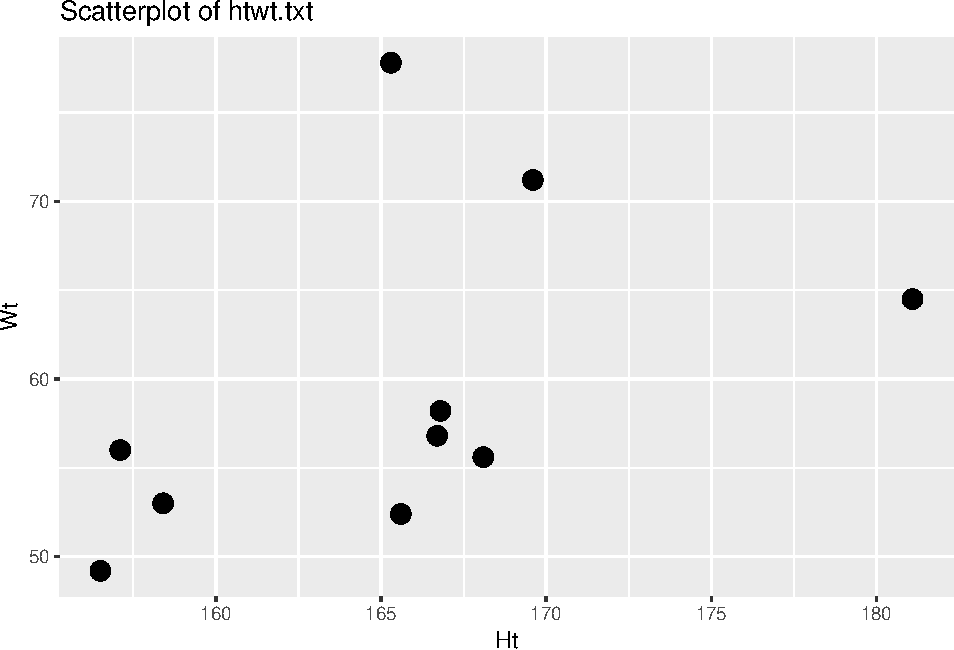
\includegraphics{Assignment_1_files/figure-latex/unnamed-chunk-4-1.pdf}
Based on the information given by this scatterplot, it is possible to
model the data using simple linear regression for the following reasons:

\begin{enumerate}
\def\labelenumi{\arabic{enumi}.}
\tightlist
\item
  There seems to be a trend between weight and height.
\item
  The tread seems to be linear.
\item
  Both weight and height exhibit reasonable variation, hence we can more
  confidently pin down the relationship between the predictor and the
  target.
\item
  The sample size of 10 is enough (barely) to perform a simple linear
  regression. 
\end{enumerate}

\paragraph{3b.}\label{b.}

\begin{verbatim}
##   Ht_mean   Wt_mean    Ht_var    Wt_var  HtWt_cov 
## 165.52000  59.47000  52.45289  81.32900  30.53178
\end{verbatim}

\begin{verbatim}
## (Intercept)          Ht 
##   -36.87588     0.58208
\end{verbatim}

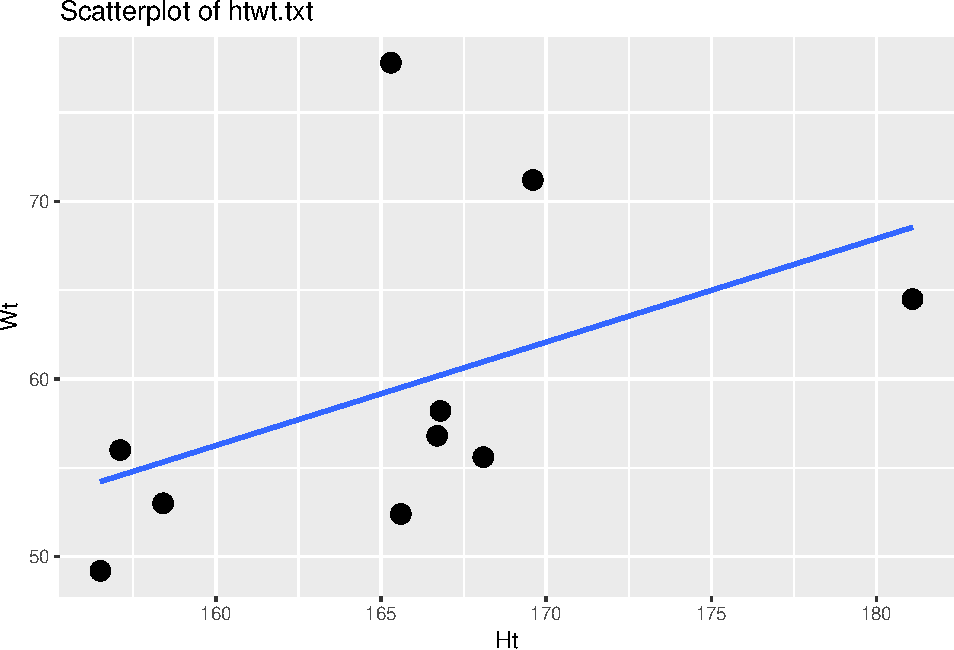
\includegraphics{Assignment_1_files/figure-latex/unnamed-chunk-5-1.pdf}

\paragraph{3c.}\label{c.}

\begin{verbatim}
##                intercept        b1
## variance       4156.7419 0.1514623
## standard error   64.4728 0.3891815
\end{verbatim}

\begin{Shaded}
\begin{Highlighting}[]
\CommentTok{#cov(b0, b1)}
\KeywordTok{unname}\NormalTok{(}\OperatorTok{-}\KeywordTok{mean}\NormalTok{(htwt}\OperatorTok{$}\NormalTok{Ht) }\OperatorTok{*}\StringTok{ }\KeywordTok{diag}\NormalTok{(}\KeywordTok{vcov}\NormalTok{(model))[}\DecValTok{2}\NormalTok{])}
\end{Highlighting}
\end{Shaded}

\begin{verbatim}
## [1] -25.07003
\end{verbatim}

\begin{Shaded}
\begin{Highlighting}[]
\KeywordTok{summary}\NormalTok{(model)}\OperatorTok{$}\NormalTok{coefficients}
\end{Highlighting}
\end{Shaded}

\begin{verbatim}
##              Estimate Std. Error    t value  Pr(>|t|)
## (Intercept) -36.87588 64.4728000 -0.5719603 0.5830589
## Ht            0.58208  0.3891815  1.4956517 0.1731089
\end{verbatim}

\paragraph{3d.}\label{d.}

\begin{Shaded}
\begin{Highlighting}[]
\KeywordTok{anova}\NormalTok{(}\KeywordTok{lm}\NormalTok{(}\DataTypeTok{data =}\NormalTok{ htwt, Wt }\OperatorTok{~}\StringTok{ }\NormalTok{Ht))}
\end{Highlighting}
\end{Shaded}

\begin{verbatim}
## Analysis of Variance Table
## 
## Response: Wt
##           Df Sum Sq Mean Sq F value Pr(>F)
## Ht         1 159.95 159.947   2.237 0.1731
## Residuals  8 572.01  71.502
\end{verbatim}

\begin{itemize}
\tightlist
\item
  Since the F value is low and p-value greater than .05, there is a high
  probability that \(\beta_{1}\) is zero and \(b_{1}\) isn't zero is
  simply due to chance.
\item
  The p-value of ANOVA and p-value of \(b_{1}\) in t-test equats.
\end{itemize}

\paragraph{\texorpdfstring{4a. }{4a.  }}\label{a.-1}

\begin{Shaded}
\begin{Highlighting}[]
\NormalTok{oldfaith_model <-}\StringTok{ }\KeywordTok{lm}\NormalTok{(}\DataTypeTok{data =}\NormalTok{ oldfaith, Interval }\OperatorTok{~}\StringTok{ }\NormalTok{Duration)}
\KeywordTok{summary}\NormalTok{(oldfaith_model)}\OperatorTok{$}\NormalTok{coefficients}
\end{Highlighting}
\end{Shaded}

\begin{verbatim}
##               Estimate Std. Error  t value     Pr(>|t|)
## (Intercept) 33.9878076 1.18121714 28.77355 6.133342e-84
## Duration     0.1768629 0.00535212 33.04540 1.624248e-96
\end{verbatim}

\[
\begin{align*}
\mathrm{\hat{Interval}} = 33.9878076 
    &+ 0.1768629\;  \mathrm{Duration}    \\
\end{align*}
\]

\begin{itemize}
\tightlist
\item
  The \(b_{1}\) is 0.1768629. This means for every second increase in
  the current eruption, the wait time will increase by 0.1768629 minute.
\end{itemize}

\paragraph{\texorpdfstring{4b. }{4b.  }}\label{b.-1}

\begin{Shaded}
\begin{Highlighting}[]
\KeywordTok{predict}\NormalTok{(oldfaith_model, }\DataTypeTok{newdata=}\KeywordTok{list}\NormalTok{(}\DataTypeTok{Duration=}\DecValTok{250}\NormalTok{), }\DataTypeTok{interval=}\StringTok{"confidence"}\NormalTok{, }\DataTypeTok{level=}\NormalTok{.}\DecValTok{95}\NormalTok{)}
\end{Highlighting}
\end{Shaded}

\begin{verbatim}
##        fit      lwr      upr
## 1 78.20354 77.36915 79.03794
\end{verbatim}

\paragraph{\texorpdfstring{4c. }{4c.  }}\label{c.-1}

\begin{Shaded}
\begin{Highlighting}[]
\KeywordTok{predict}\NormalTok{(oldfaith_model, }\DataTypeTok{newdata=}\KeywordTok{list}\NormalTok{(}\DataTypeTok{Duration=}\DecValTok{250}\NormalTok{), }\DataTypeTok{interval=}\StringTok{"prediction"}\NormalTok{, }\DataTypeTok{level=}\NormalTok{.}\DecValTok{95}\NormalTok{)}
\end{Highlighting}
\end{Shaded}

\begin{verbatim}
##        fit      lwr      upr
## 1 78.20354 66.35401 90.05307
\end{verbatim}

\paragraph{\texorpdfstring{5. }{5.  }}\label{section}

\begin{itemize}
\tightlist
\item
  When there is no variation in the predictor variable, the denominator
  of the closed-form formula of \(b_{1}\) is zero. Thereby \(b_{1}\) is
  not defined. Regression tries to answer the question: How does y
  change, on average, when X changes by one unit? This question cannot
  be answered if X doesn't change.
\end{itemize}


\end{document}
